%----------------------------------------------------------------------------------------
%	PACKAGES AND OTHER DOCUMENT CONFIGURATIONS
%----------------------------------------------------------------------------------------

\documentclass[final, 36 pt]{beamer}

\usepackage[size = a0, scale=1.05]{beamerposter} % Use the beamerposter package for laying out the poster
\usepackage{pdfpages}
\usepackage{amsmath,amsthm,amssymb}
\usepackage{tikz}
\usepackage{pstricks}
\usepackage{ragged2e}
\usepackage{mathrsfs}
\usepackage{microtype}
\usepackage{bbm}
\usepackage{graphicx, wrapfig, subcaption, setspace, booktabs}
\usepackage{tabularx}
\usepackage{listings}
\usepackage{xcolor}
\usepackage{longtable}
%\usepackage{titlesec}
\usepackage{url, lipsum}
\usepackage{hyperref,bookmark}
\usepackage[T1]{fontenc}
\usepackage{amssymb}
%\usepackage{orcidlink}
\usepackage{tabularx}
\usepackage{listings}
\usepackage{xcolor}
\usepackage{longtable}
\usepackage{setspace}
\usepackage{float}
\usepackage{multirow}
\usepackage{svg}
\usepackage[ruled,linesnumbered]{algorithm2e}
%\renewcommand{\familydefault}{\sfdefault}
\usepackage{helvet}
\renewcommand{\familydefault}{\sfdefault}
\usepackage{sansmath} % Enables turning on sans-serif math mode, and using other environments
\sansmath % Enable sans-serif math for rest of document

\usepackage[math]{blindtext}


\usetheme{confposter} % Use the confposter theme supplied with this template

\setbeamercolor{block title}{fg=ngreen,bg=white} % Colors of the block titles
\setbeamercolor{block body}{fg=black,bg=white} % Colors of the body of blocks
\setbeamercolor{block alerted title}{fg=white,bg=dblue!70} % Colors of the highlighted block titles
\setbeamercolor{block alerted body}{fg=black,bg=dblue!10} % Colors of the body of highlighted blocks
% Many more colors are available for use in beamerthemeconfposter.sty

%-----------------------------------------------------------
% Define the column widths and overall poster size
% To set effective sepwid, onecolwid and twocolwid values, first choose how many columns you want and how much separation you want between columns
% In this template, the separation width chosen is 0.024 of the paper width and a 4-column layout
% onecolwid should therefore be (1-(# of columns+1)*sepwid)/# of columns e.g. (1-(4+1)*0.024)/4 = 0.22
% Set twocolwid to be (2*onecolwid)+sepwid = 0.464
% Set threecolwid to be (3*onecolwid)+2*sepwid = 0.708

\newlength{\sepwid}
\newlength{\onecolwid}
\newlength{\twocolwid}
\newlength{\threecolwid}
\setlength{\paperwidth}{48in} % A0 width: 46.8in
\setlength{\paperheight}{36in} % A0 height: 33.1in
\setlength{\sepwid}{0.024\paperwidth} % Separation width (white space) between columns
\setlength{\onecolwid}{0.22\paperwidth} % Width of one column
\setlength{\twocolwid}{0.464\paperwidth} % Width of two columns
\setlength{\threecolwid}{0.708\paperwidth} % Width of three columns
\setlength{\topmargin}{-0.5in} % Reduce the top margin size

\setbeamertemplate{caption}[numbered]
%-----------------------------------------------------------

\usepackage{graphicx}  % Required for including images

\usepackage{booktabs} % Top and bottom rules for tables

%----------------------------------------------------------------------------------------
%	TITLE SECTION 
%----------------------------------------------------------------------------------------

\title{CO\textsubscript{2} and Cost Impacts of a Microgrid  with Electric Vehicle \\Charging Infrastructure: a Case Study in Southern California} % Poster title

\author{Luis Fernando Enriquez-Contreras, Matthew Barth, Sadrul Ula} % Author(s)

\institute{College of Engineering, Center for Environmental Research \& Technology \\ University of California, Riverside} % Institution(s)

%----------------------------------------------------------------------------------------

\begin{document}
\bf
\addtobeamertemplate{headline}{} 
{\begin{tikzpicture}[remember picture, overlay]
		\node [anchor=north east, inner sep=4cm]  at (current page.north east)
		{
\includegraphics[height=4cm]{Fig/CECERT_logo_crop.pdf}};
\end{tikzpicture}}
\addtobeamertemplate{headline}{} 
{\begin{tikzpicture}[remember picture, overlay]
		\node [anchor=north west, inner sep=3cm]  at (current page.north west)
		{
\includegraphics[height=7cm]{Fig/ucr_logo.pdf}};
\end{tikzpicture}}
\addtobeamertemplate{block end}{}{\vspace*{2ex}} % White space under blocks
\addtobeamertemplate{block alerted end}{}{\vspace*{2ex}} % White space under highlighted (alert) blocks

\setlength{\belowcaptionskip}{2ex} % White space under figures
\setlength\belowdisplayshortskip{2ex} % White space under equations

\begin{frame}[t] % The whole poster is enclosed in one beamer frame

\begin{columns}[t] % The whole poster consists of three major columns, the second of which is split into two columns twice - the [t] option aligns each column's content to the top

\begin{column}{\sepwid}\end{column} % Empty spacer column

\begin{column}{\onecolwid} % The first column

%----------------------------------------------------------------------------------------
%	OBJECTIVES
%----------------------------------------------------------------------------------------
\begin{alertblock}{Abstract}
	\begin{itemize}
		\item This paper presents a case study at the University of California, Riverside (UCR) that evaluates the effectiveness of different transportation-based microgrid configurations in reducing both carbon dioxide (CO\textsubscript{2}) emissions and electricity costs
		\item Electric costs were also compared to determine the financial savings potential for the consumer
		\item The results demonstrate that a peak-shaving transportation-microgrid strategy can effectively reduce CO\textsubscript{2} emissions in the range of 24\% to 38\% and costs from \$27,000 to \$29,000 per year
		\item  Careful consideration should be given to battery sizing, as peak-shaving has diminishing returns
	\end{itemize}
	%	As an important part of Intelligent Transportation Systems (ITS), this paper presents a case study at the University of California, Riverside (UCR) that evaluates the effectiveness of different transportation-based microgrid configurations in reducing both carbon dioxide (CO\textsubscript{2}) emissions and electricity costs. CO\textsubscript{2} emissions are calculated using high-resolution California Independent System Operator (CAISO) CO\textsubscript{2} emissions data to accurately assess the environmental impact of each setup. Electric costs were also compared to determine the financial savings potential for the consumer. The results demonstrate that a peak-shaving transportation-microgrid strategy can effectively reduce CO\textsubscript{2} emissions in the range of 24\% to 38\% and costs from \$27,000 to \$29,000 per year, even when considering the additional demand from 12 vehicles charging daily at the building. However, careful consideration should be given to battery sizing, as peak-shaving has diminishing returns. Doubling the battery size may only provide an additional savings of \$2,000 per year with a negligible reduction in emissions. This highlights the importance of optimizing battery capacity to maximize cost-effectiveness and environmental impact.
\end{alertblock}
%----------------------------------------------------------------------------------------
%	INTRODUCTION
%----------------------------------------------------------------------------------------
\begin{alertblock}{Purpose and Contributions}
	\begin{itemize}
		\item This research holds significant implications for the advancement of intelligent transportation systems, as it aims to address the economic needs of EV charging infrastructure owners and determine the optimal configuration that benefits both EV owners and the environment by minimizing greenhouse gas emissions
		\item This paper delves into the impacts of transportation-microgrids equipped with Level 2 and Level 3 charging on the behavior of microgrids, associated electricity costs, and CO\textsubscript{2} emissions within the context of southern California
		\item The simulations are conducted using OpenModelica, a dynamic modeling and simulation environment
		\item This study distinguishes itself from previous research in many ways, including employing a higher time resolution for calculating CO\textsubscript{2} emissions that is measured every 15 minutes
	\end{itemize}
\end{alertblock}

\begin{block}{}
		\begin{figure}[!htb] 		
		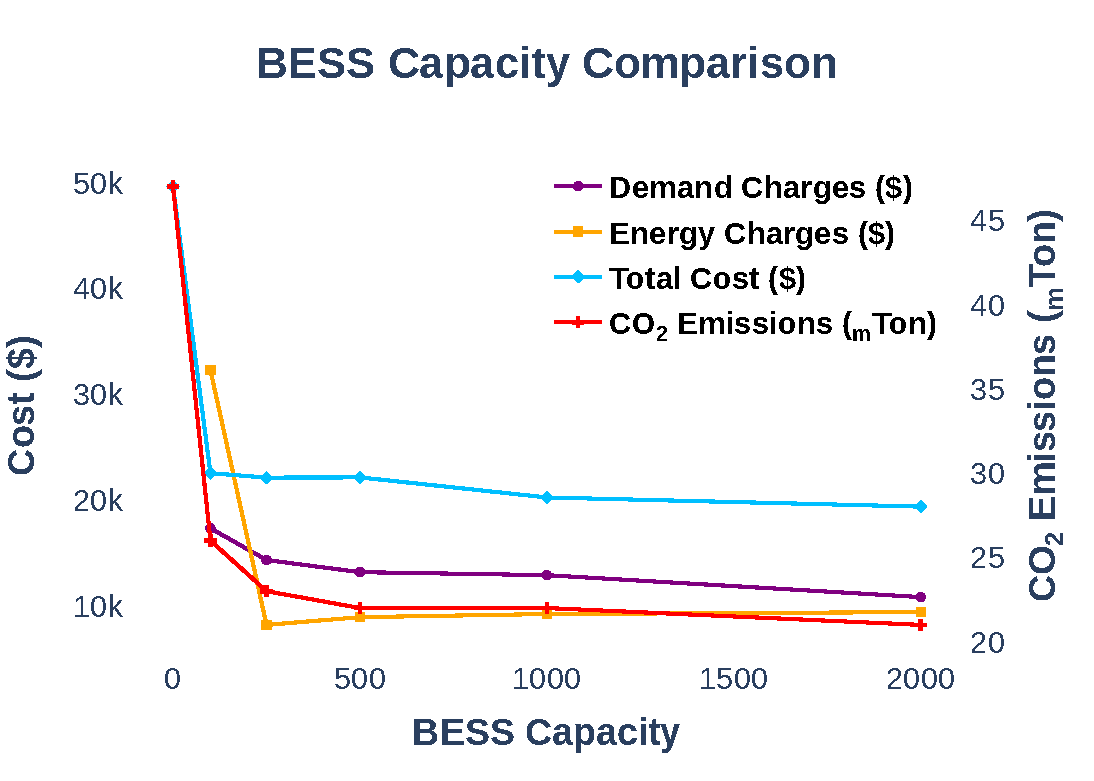
\includegraphics[width=\linewidth]{Fig/bess_capacity_comparison_large_font}
		\caption{\large Cost and CO\textsubscript{2} Emissions for Different Battery Capacities. A BESS capacity of 250 -500 kWh is ideal for the lowering costs and CO\textsubscript{2} emissions without with less diminishing returns in savings. }
		\label{fig:besscapacitycomparison}		
	\end{figure}
\end{block}

%\begin{block}{Transportation-microgrids Mindmap}	
%	\begin{figure}
%		\centering
%		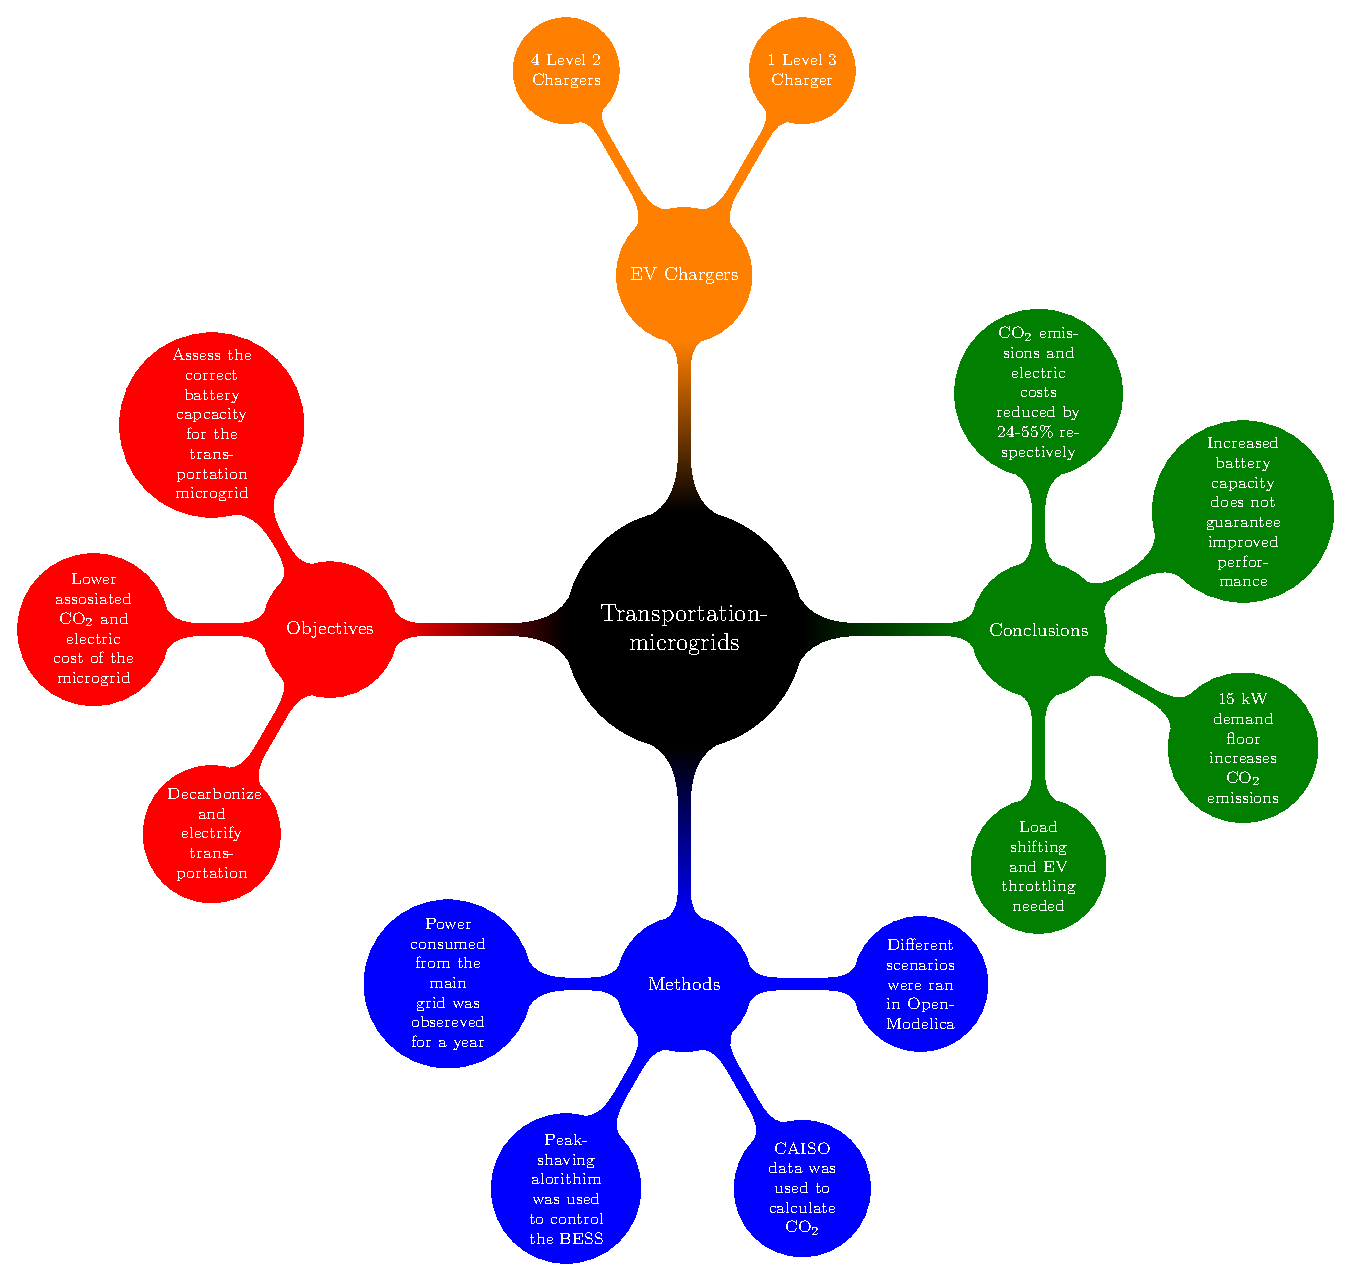
\includegraphics[width=0.7\linewidth]{Fig/paper_mindmap}
%		\caption{}
%		\label{fig:papermindmap}
%	\end{figure}	
%\end{block}

\end{column} % End of the first column

\begin{column}{\sepwid}\end{column} % Empty spacer column

\begin{column}{\twocolwid} % The second column

%----------------------------------------------------------------------------------------
%	Setup
%----------------------------------------------------------------------------------------

\begin{block}{Microgrid Architecture}
	\begin{figure}[!htb] 		
		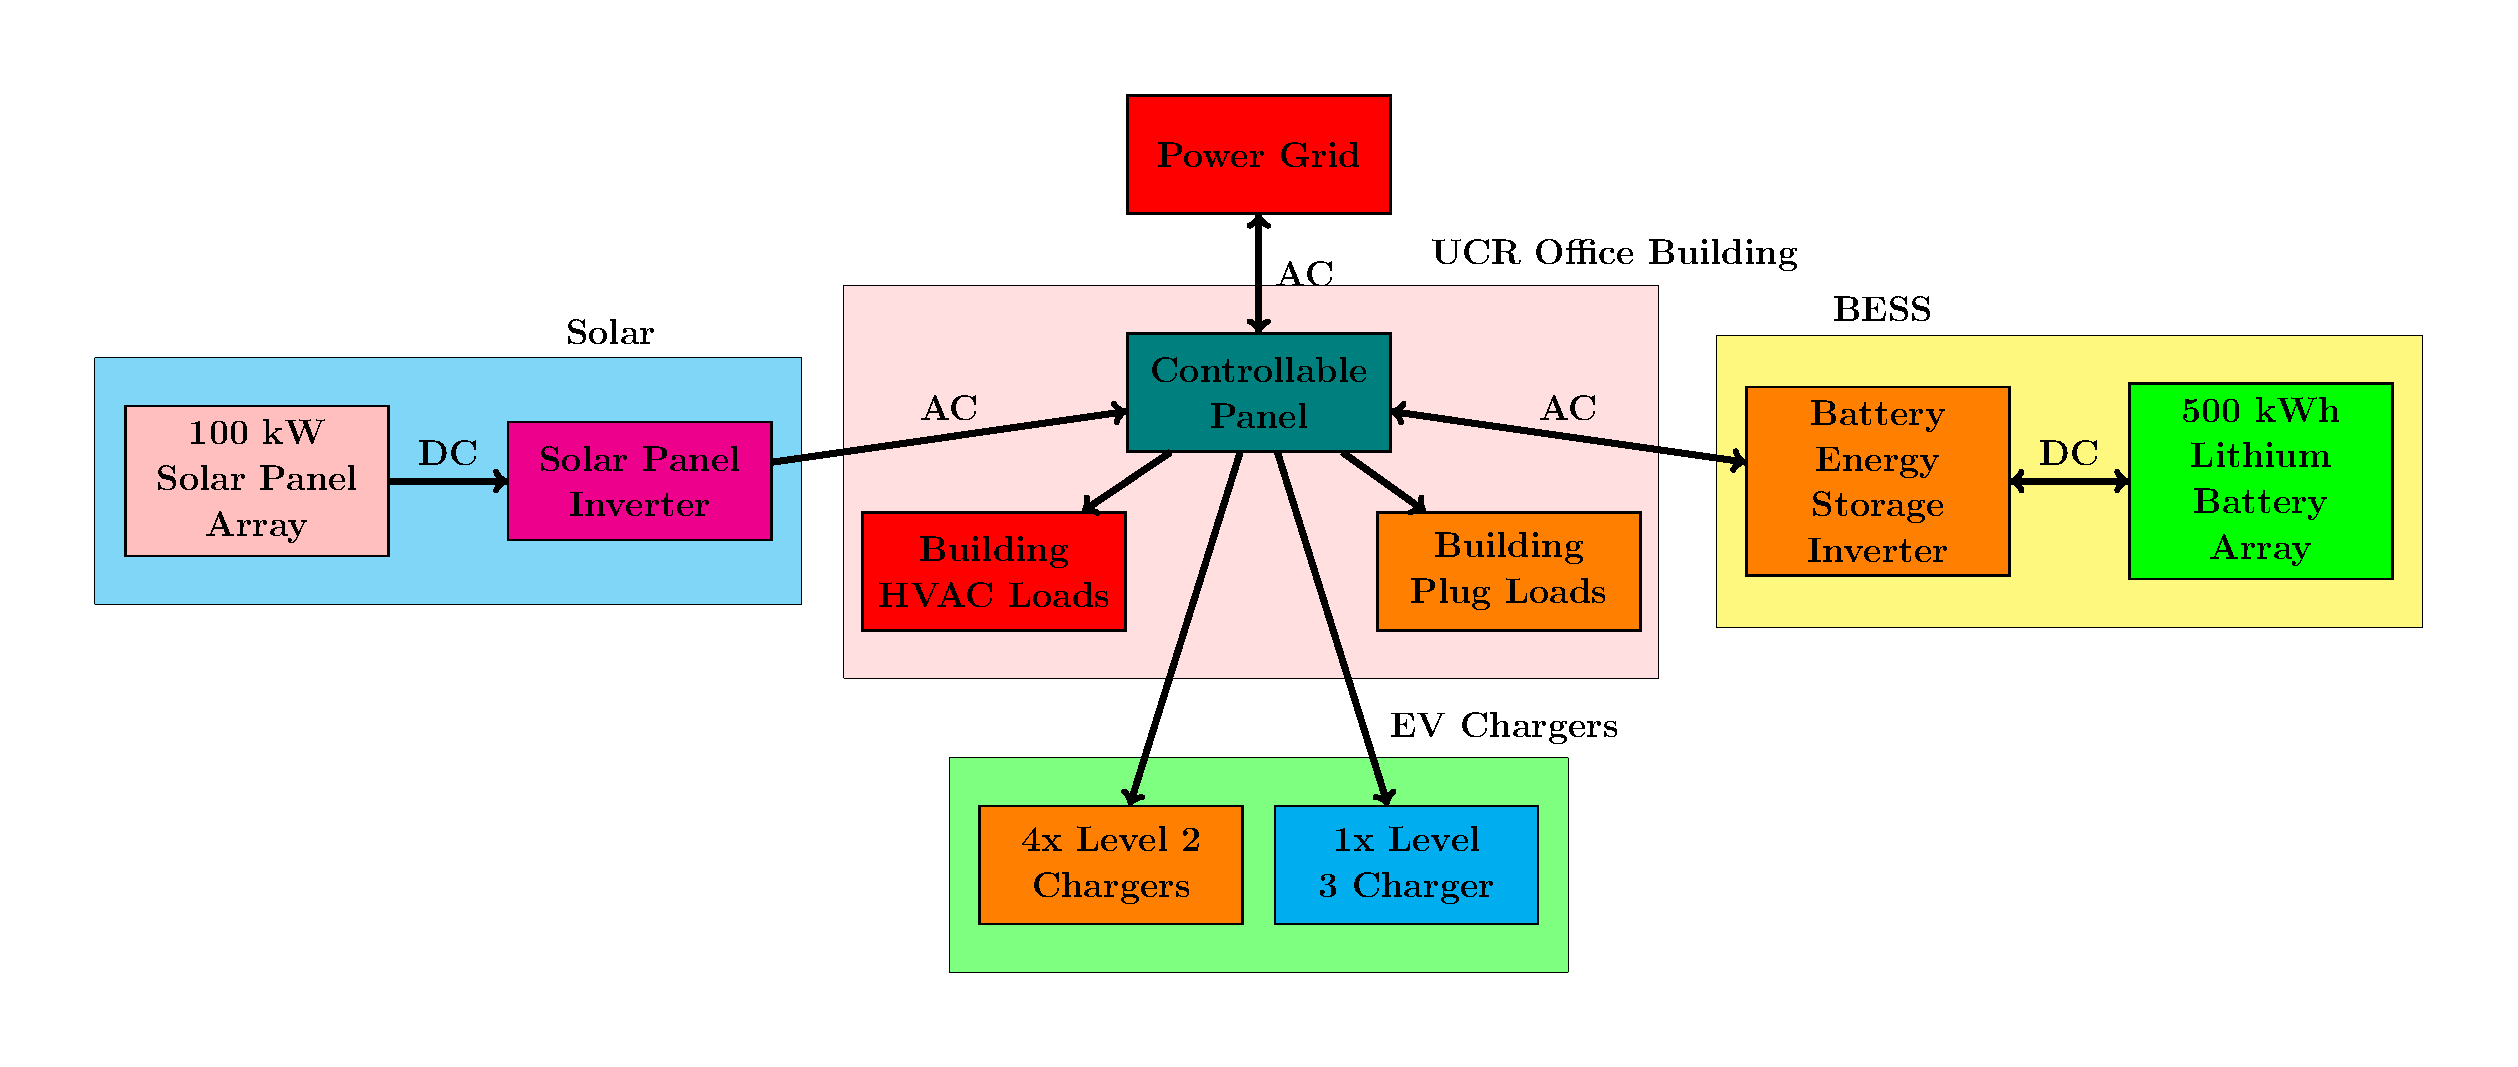
\includegraphics[width=\linewidth]{Fig/power_system_setup_modelica_large}
		\caption{Microgrid Architecture of our Case Study Example BESS: Battery Energy Storage System}
		\label{fig:powersystemsetupfull}
	\end{figure}
\end{block}

\begin{block}{Simulated Scenarios of the UCR Microgrid using Different Layouts}
	
	\begin{table}
		\caption{}
		\centering
		\begin{tabularx}{\linewidth}{l | l}
\toprule
 Scenario &  \\
\midrule
		1  & Standard Building with no EV Chargers\\
        2 & Standard Building with Level 2 and Level 3 Charging\\
        3 & Microgrid Building with 100 kW Solar, 500 kWh BESS, No EV Charging \\
        4 & Microgrid Building with 100 kW Solar, 100 kWh BESS, Level 2, and Level 3 Charging\\
        5 & Microgrid Building with 100 kW Solar, 250 kWh BESS, Level 2, and Level 3 Charging\\
        6 & Microgrid Building with 100 kW Solar, 500 kWh BESS, Level 2, and Level 3 Charging\\
        7 & Microgrid Building with 100 kW Solar, 1 MWh BESS, Level 2, and Level 3 Charging\\
        8 & Microgrid Building with 100 kW Solar, 1 MWh BESS, Level 2, and Level 3 Charging\\
\bottomrule
\end{tabularx}

		\label{tab:scenarios}
	\end{table}
	
\end{block}

\begin{block}{Microgrid Utility Electricity Prices and Associated CO\textsubscript{2} Emissions Output under Different Scenarios}
	\begin{table}
		\caption{}
		\centering
		\large
		\input{Table/kw_kwh_CO2_run_4.tex}
		\label{tab:emissions}
	\end{table}
\end{block}




%\begin{block}{EV Charging Simulations}
%	\begin{figure}
%		\centering
%		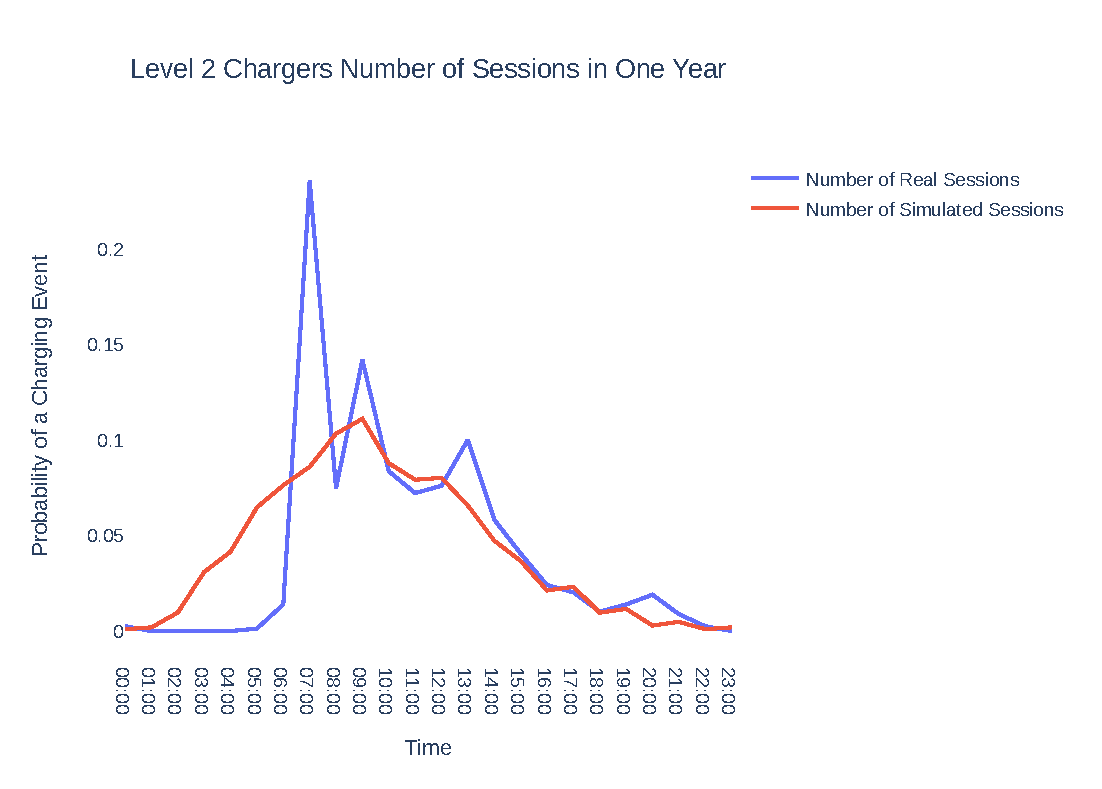
\includegraphics[width=\linewidth]{Fig/l2_avg_day_rand_poisson_1_hour_pdf}
%		\caption{Validation of the Level 2 EV Charger Stochastic Process that Compares the Probability Density Function of Actual Charging Data to the Poisson Process}
%		\label{fig:l2avgdayrandpoisson1hourpdf}
%	\end{figure}
%	
%\end{block}


%----------------------------------------------------------------------------------------

\end{column} % End of the second column

\begin{column}{\sepwid}\end{column} % Empty spacer column

\begin{column}{\onecolwid} % The third column
	\begin{figure}
	\centering
	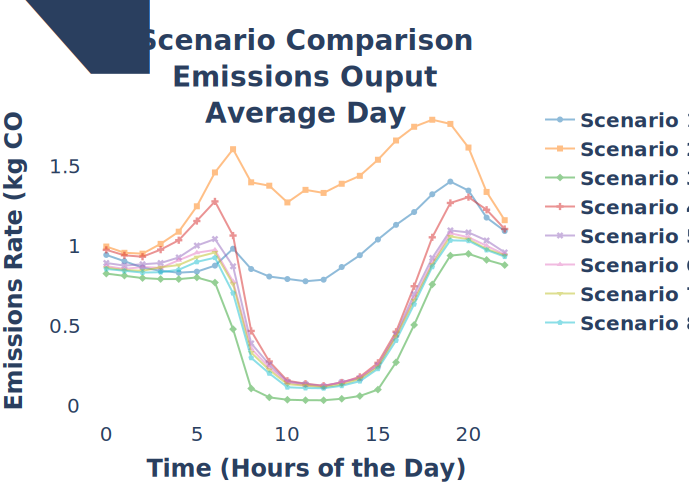
\includegraphics[width=\linewidth]{Fig/emissions_scenario_comparison_run_3_large_font}
	\caption{\large Microgrid CO\textsubscript{2} Emissions Outputs Averages During Times of Day. Adding a microgrid significantly reduces CO\textsubscript{2} Emissions compared to the non-microgrid scenarios 1 and 2.}
	\label{fig:emissionsscenariocomparison}
\end{figure}

%----------------------------------------------------------------------------------------
%	CONCLUSION
%----------------------------------------------------------------------------------------

\begin{alertblock}{Conclusions and Future Work}
	\begin{itemize} 
		\item Transportation-microgrids offer significant economic and environmental benefits
		\begin{itemize} 
			\item Estimated annual savings of \$8,000-\$10,000 compared to conventional systems
			\item Annual savings of \$27,000-\$29,000 compared to buildings with EV chargers but no microgrid
			\item 24\% - 38\% reduction in CO\textsubscript{2} emissions compared to conventional buildings
			\item 45\% - 55\% reduction in CO\textsubscript{2} emissions compared to buildings with EV chargers and no microgrid
		\end{itemize}
		\item Increased battery capacity does not guarantee improved performance
		\begin{itemize} 
			\item Increased capacity improves performance but not proportionally to the cost
			\item Large capacity needed for challenging situations may not be cost-effective 
		\end{itemize}
		\item 15 kW demand price floor discourages zero net load
		\begin{itemize} 
			\item Discourages zero net load in peak shaving setups, increasing CO\textsubscript{2} emissions
		\end{itemize}
		\item Future Work
		\begin{itemize} 
			\item Optimizing electric costs and CO\textsubscript{2} emissions through throttling charging, maximizing solar energy use, and minimizing grid draw during peak CO\textsubscript{2} emissions times
			\item Assessing the impact of California's new net energy metering policy
		\end{itemize}
	\end{itemize}
\end{alertblock}


%----------------------------------------------------------------------------------------
%	ACKNOWLEDGEMENTS
%----------------------------------------------------------------------------------------

\setbeamercolor{block title}{fg=red,bg=white} % Change the block title color

\begin{block}{Acknowledgements}

I would like to give a special thanks to the CE-CERT staff, the Dwight David Eisenhower Transportation Fellowship Program, and my family who have supported me throughout my research and without them this contribution would not be possible. \\

\end{block}


%----------------------------------------------------------------------------------------
%----------------------------------------------------------------------------------------
%	CONTACT INFORMATION
%----------------------------------------------------------------------------------------

\setbeamercolor{block alerted title}{fg=black,bg=norange} % Change the alert block title colors
\setbeamercolor{block alerted body}{fg=black,bg=white} % Change the alert block body colors

\begin{alertblock}{Contact Information}
	
	\begin{itemize}
		\item Researcher: Luis Fernando Enriquez-Contreras
		\item Web: \href{https://www.cert.ucr.edu/transportation-systems-vehicle-infrastructure-interaction}{https://www.cert.ucr.edu/transportation-systems-vehicle-infrastructure-interaction}
		\item Email: \href{lenri001@ucr.edu}{lenri001@ucr.edu}
		\item Phone: +1 (909) 763 1899
	\end{itemize}
	
\end{alertblock}

\begin{center}
	\begin{tabular}{ccc}
		%\includegraphics[width=0.4\linewidth]{logo.png} & \hfill & %\includegraphics[width=0.4\linewidth]{logo.png}
	\end{tabular}
\end{center}

\end{column} % End of the third column

\end{columns} % End of all the columns in the poster

\end{frame} % End of the enclosing frame

\end{document}